
% JuliaCon proceedings template
\documentclass{juliacon}

\usepackage{amsmath}
\usepackage{float}

\usepackage[super]{nth}

\setcounter{page}{1}

\begin{document}

% **************GENERATED FILE, DO NOT EDIT**************

\title{HydroPowerModels.jl: A Julia/JuMP Package for Hydrothermal Economic Dispatch Optimization}

\author[1, 2]{Andrew W. Rosemberg}
\author[1, 2]{Alexandre Street}
\author[1, 2]{Joaquim D. Garcia}
\author[1, 3]{Thuener Silva}
\author[1, 3]{\\ Davi M. Valladão}
\author[4]{Oscar Dowson}
\affil[1]{Laboratory of Applied Mathematical Programming and Statistics (LAMPS)}
\affil[2]{Department of Eletrical Engineering, PUC-RIO}
\affil[3]{Department of Industrial Engineering, PUC-RIO}
\affil[4]{Department of Industrial Engineering, Northwestern University, Evanston}

\keywords{Julia, Optimization, Energy, Stochastic}



\maketitle

\begin{abstract}

\textit{HydroPowerModels.jl} is a Julia package for solving multistage, steady-state, hydro-dominated, power network optimization problems with stochastic dual dynamic programming (SDDP). Our state-of-the-art open source tool is flexible enough for practitioners in the electrical sector to test new ideas in an efficient way. This tool was made possible by the Julia language and the surrounding ecosystem of packages. We use \textit{JuMP}, a package for mathematical programming modeling; \textit{PowerModels.jl}, a JuMP-extension for power network optimization; and \textit{SDDP.jl}, another extension that implements the SDDP algorithm.

\end{abstract}

\section{Introduction}

The hydrothermal dispatch problem is important for the planning and operation of hydro-dominated electrical systems such as the Brazilian national grid. The objective is to coordinate generation, energy distribution, and hydro-storage management in order to minimize the cost of operation. In this context, the hydrothermal dispatch problem is a medium-term planning problem where uncertainties related to the hydrology (i.e., rainfall and other inflows) of the hydroelectric plants and consumer-demand have fundamental importance. Generation takes two main forms: i) hydro-generation with a low marginal cost, and ii) thermal-generation, with a high marginal cost. However, in hydro-dominated systems such as Brazil, there is often insufficient capacity of thermal generation to meet demand. Thus, the system-operator faces a trade-off between using water for cheap generation in the present, against conserving water for future periods of drought. Because of this trade-off, the hydrothermal dispatch problem is often modeled as a multistage stochastic problem \cite{pereira1991multi,maceiral2018twenty,terlaky_marginal_2017}.
 %\vskip 6pt

Solving multistage stochastic programs, however, is a challenging numerical problem. The solution of the problem is intractable and common approximations such as stochastic dynamic programming \cite{bellman1966dynamic} \cite{bertsekas1995dynamic} can suffer from high dimensionality (frequently referred as the curse of dimensionality). One method that partially overcomes the curse of dimensionality is the stochastic dual dynamic programming algorithm of ~\cite{pereira1991multi}.

% <review @Lukrosz>
% I was taught not to use apostrophes in articles. However, I have seen other articles in different journals where apostrophes are used. Therfore, I encourage you not to use them but the decision is up to you.
% </review>
A number of programs implementing SDDP are in-use around the world, ranging from unpublished implementations in academic institutions to professional software such as the product developed by PSR, a software and consulting company, also called \textit{SDDP}\footnote{Note that the ``SDDP'' acronym is used to denote a software product, the original algorithm of \cite{pereira1991multi}, and a more general class of algorithms inspired by the original SDDP algorithm.} \cite{psr_software_2019}. However, until recently, there was no fast, reliable, and open-source implementation of the SDDP algorithm. Without such a tool, researchers and practitioners have not had a common ground for the discussion and analysis of different hydrothermal dispatch formulations and their solutions.

The objective of this work is to build an open source tool, called \href{https://github.com/andrewrosemberg/HydroPowerModels.jl}{\textit{HydroPowerModels.jl}}, that can be this common ground. \textit{HydroPowerModels.jl} can be used to assess the impact of modeling choices during the planning of a hydrothermal power system. These choices include the usage of different network formulations, the consideration of different risk measures, and the planning horizons for uncertain future costs. Addressing these issues provides the research community and the energy industry with a powerful tool for the efficient design of hydrothermal power systems.

To develop a tool that can be used by both researchers and industry professionals, we take advantage of the Julia language~\cite{bezanson2017julia} and two main packages: \href{https://github.com/lanl-ansi/PowerModels.jl}{\textit{PowerModels.jl} ~\cite{8442948}, which implements power flow models for electrical dispatch, \href{https://github.com/odow/SDDP.jl}{\textit{SDDP.jl}} ~\cite{dowson_sddp.jl}, which implements the stochastic dual dynamic programming algorithm}. Both \textit{PowerModels.jl} and \textit{SDDP.jl} handle their respective optimization models through \href{https://github.com/JuliaOpt/JuMP.jl}{\textit{JuMP.jl}} \cite{DunningHuchetteLubin2017}, a Julia package for mathematical optimization. \textit{JuMP.jl} makes it simple to write complex optimization problems and solve them with numerous solvers. \textit{HydroPowerModels.jl} takes advantage from the fact that \textit{PowerModels.jl} and \textit{SDDP.jl} were not only developed in Julia, but also deeply rely on \textit{JuMP.jl} to build and solve mathematical optimization problems. \textit{SDDP.jl} is used to specify the hydro storage dynamics and stochastics of inflows, renewables and loads. \textit{PowerModels.jl} is used to provide multiple network dispatch formulations as a starting point for the \textit{HydroPowerModels.jl} formulation that couples the electrical constraints with hydro constraints and uncertainty.

The next sections are organized as follows: 1) A brief understanding of multistage stochastic problems and decisions under uncertainty; 2) A presentation of the problem's modeling formulation and specification; 3) Different simplifications of the model; 4) An explanation of the solution method (SDDP); 5) A comparison of existing alternative solution implementations and listing of the proposed package functionalities; 6) A case study to clarify usage.

\section{Multistage Stochastic Optimization}
\label{sec:multistochopt}

Stochastic Programming (SP) \cite{shapiro2009lectures} is a branch of optimization under uncertainty, where the realization of some random variables ($\omega$) influence the problem's conditions and consequently the optimal decisions. Uncertainty relates to the probability distributions of parameters and may be incorporated to the problem in various manners. 

One class of simple stochastic programs is known as a two-stage problem with recourse. It can be formulated as follows:

\begin{equation*}
\nth{1} \text{ Stage} \left\{
\begin{aligned}
& \underset{x}{\text{min}}
& & c^T x + \overbrace{\rho[Q(x, \omega)]}^{\mathcal{Q}(x)} \\
& \text{s.t.}
& & x \in \mathcal{X}
\end{aligned}
\right.
\end{equation*}

\begin{equation*}
\nth{2} \text{ Stage} \left\{
\mathcal{Q}(x, \omega) = \left\{
\begin{aligned}
& \underset{u}{\text{min}}
& & g^T u \\
& \text{s.t.}
& & A u = b(\omega)- E x \\
& & & u \in \mathcal{U} 
\end{aligned}
\right. \right\}.
\end{equation*}

The objective of the first stage is composed of an \textit{immediate cost} term $c^T x$ and a \textit{cost-to-go function} $\mathcal{Q}(x)$. $\mathcal{Q}$ is a function of some decision variables of the first stage $x$ that fix the state of the second stage (its feasible region). These variables are called \textit{state variables}. First stage decisions are made under uncertainty, while the decision variables of the second stage $u$ are chosen after the realization of the variable $\omega$ (under a deterministic scope) and are so called \textit{recourse variables}. The function $\rho$ is known as a \textit{risk measure} \cite{artzner1999coherent} and is commonly assumed to be the expectation operator $\mathbb{E}$.

The goal of this problem is to find an optimal stage decision $x$ and an optimal second-stage decision $u$ for each realization of $\omega$ conditioned on $x$. Collectively, this set of decisions is known as a \textit{policy}.

The two-stage problem discussed above naturally extends to a \textit{multistage} problem via recursion. A multistage stochastic program with $T$ stages can be formulated as follows:

 \begin{equation*}
    \begin{aligned}[t]
        \underset{x_1 \in \mathcal{X}_1}{\text{min}}
        & f_1(x_1) + \\ 
        & \qquad \rho[ \underset{x_2 \in \mathcal{X}_2(x_1,\omega_{2})}{\text{inf}} f_2(x_2,\omega_{2}) + \\ 
        & \qquad \qquad \rho[... + \rho[\underset{x_T \in \mathcal{X}_T(x_{T-1},\omega_{T})}{\text{inf}} f_T(x_T,\omega_{T})]...]] \\
    \end{aligned}
\end{equation*}

Assuming the problem is linear, we have:

 \begin{equation*}
    \begin{aligned}
        & \mathcal{X}_{t}(x_{t-1},\omega) = \big\{ x_t \geq 0 : A_t x_t = b_t(\omega)- E_t x_{t-1} \big\} \\
        & f_t(x_t,\omega) = c_t^T x_t
    \end{aligned}
\end{equation*}

In this setting, the uncertain data $\omega_1 , ..., \omega_T$ is revealed gradually over time. The sequence $\omega_t \in \mathbb{R}^{d_t}$ of data vectors is viewed as a stochastic process, i.e., as a sequence of random variables with a specified probability distribution.

Just like in the two stage problem, there are state variables at every stage that partially impact the objective through the risk measure of the subsequent stages optimal values. The policy optimized by this problem is a mapping from the realized stochastic process to the decisions for each stage. 

Using dynamic programming \cite{bellman1966dynamic}, the nested formulation of a multistage stochastic program may be represented by the following Bellman recursion for each stage:

 \begin{equation*}
    Q_t(x_{t-1}, \omega_{t}) = \left\{
    \begin{aligned}
    & \underset{x_t}{\text{min}} 
    & & c_t^T x_{t} + \rho_{t+1}[Q_{t+1}(x_{t}, \omega_{t+1})]  \\
    & \text{s.t.} \notag
    & & A_t x_t = b_t(\omega_{t})- E_t x_{t-1} \qquad [\pi_t(\omega_{t})]\\
    & & & x_t \geq 0 \\
    \end{aligned}
    \right\}
\end{equation*}

For the purpose of simplicity, we assume that $\mathcal{Q}_{T+1}(\cdot, \cdot) = 0$.

In these equations, the optimal value at stage $t$ depends on previous decision $x_{t-1}$ and the realization of the data process $\omega_t$. Finally, the optimal value of the first stage problem gives the optimal value of the corresponding multistage problem. 

\section{The Hydrothermal Dispatch Problem}
\label{sec:problemformulation}
%
The hydrothermal dispatch problem is a multistage stochastic optimization problem that comprises an optimal power flow (OPF) problem and the hydro storage management for multiple periods and scenarios. 

Introduced by \cite{carpentier1962contribution}, the OPF problem extends the economic dispatch problem, where the goal is to plan the operation of an electrical power system by determining the contribution of available energy sources in supplying demands, to include constraints representing the power flow equations, resulting in a more realistic model of the dispatch. 

Since its introduction, the OPF problem has received additional constraints to better represent power systems. The adopted version of the \textit{PowerModels.jl} package, is a AC Optimal Power Flow (AC-OPF) problem. The AC Power Flow constraints implement voltage bounds, generation bounds, nodal conservation of power, power flow on lines and thermal limit of the lines (power flow limit) for an alternating current system. Different from original OPF formulations, support was also added for multiple load and shunt components on each bus together with a line charging that supports conductance and asymmetrical values.

Besides the modifications from \textit{PowerModels.jl}, deficit variables to work as slack to the attendance of each load have frequently been used by the electrical sector and will be incorporated in our package. This variables allow a more detailed evaluation of the cost of not attending some demands. 

The optimal dispatch tries to find the most economic use of system resources and is the objective function of an OPF. However, in a hydrothermal power system, where water is a main resource and its inflow is uncertain, risk averse planning is an important task to ensure the lowest cost operation. The necessary hydro storage management to attend demand during periods of scarcity adds an extra layer of decisions and constraints.

Reservoir operation is a problem composed by the balance of incoming and outgoing flow of water as well as its usage to generate power. Since many storage facilities are linked through rivers, this problem may be simply viewed as a directed flow graph where each node in the graph represents a storage reservoir. A constraint binds the power generation of generators using water as fuel to the outflow of the respective storage. Operation is also restricted by the limits of reservoir volume and outflow.

The solution of this problem returns an operation policy representing the optimal generation and hydro management possible given the horizon studied and the scenarios considered.

As it is common for multistage problems, we will define the underlying sub-problem (i.e., $\mathcal{Q}$) that unifies the OPF problem with the hydro-thermal dispatch problem.

\subsection{The Mathematical Model}
\label{subsub:mathmodel}

Following the notation chosen by the \textit{PowerModels.jl} package, the sets and parameters used to define the sub-problem are listed with the addition of those created for the hydro storage management and the data for the state of the sub-problem:

\subsubsection*{Sets}
\begin{align*}
%
% \mbox{sets:} & \nonumber \\
& N \mbox{ - buses}\nonumber \\
& R \mbox{ - reference buses}\nonumber \\
& E, E^R \mbox{ - branches, forward and reverse orientation} \nonumber \\
& G, G_i \mbox{ - generators and generators at bus $i \in N$} \nonumber \\
& L, L_i \mbox{ - loads and loads at bus $i \in N$} \nonumber \\
& S, S_i \mbox{ - shunts and shunts at bus $i \in N$} \nonumber \\
& H, H^G \mbox{ - reservoirs and reservoirs with power generation}\nonumber \\
& H^U_h, H^{\mathfrak{S}}_h \mbox{ - upstream reservoirs out-flowing and spilling to $h\in H$ }\nonumber \\
& G^H_h \mbox{ - generator at reservoir $h\in H$}\nonumber \\
%
\end{align*}

\subsubsection*{Data}
\begin{align*}
%
% \mbox{data:} & \nonumber \\
& S^{gl}_k, S^{gu}_k \;\; \forall k \in G \nonumber \mbox{ - generator complex power bounds}\\
& c_{2k}, c_{1k}, c_{0k} \;\; \forall k \in G \nonumber  \mbox{ - generator cost components}\\
& v^l_i, v^u_i \;\; \forall i \in N \nonumber \mbox{ - voltage bounds}\\
& S^d_k \;\; \forall k \in L \nonumber \mbox{ - load complex power consumption}\\
& Y^s_{k} \;\; \forall k \in S \nonumber \mbox{ - bus shunt admittance}\\
& Y_{ij}, Y^c_{ij} \;\; \forall (i,j) \in E \nonumber \mbox{ - branch pi-section parameters}\\
& {T}_{ij} \;\; \forall (i,j) \in E \nonumber \mbox{ - branch complex transformation ratio}\\
& s^u_{ij}  \;\; \forall (i,j) \in E \nonumber \mbox{ - branch apparent power limit}\\
& i^u_{ij}  \;\; \forall (i,j) \in E \nonumber \mbox{ - branch current limit}\\
& \theta^{\Delta l}_{ij}, \theta^{\Delta u}_{ij} \;\; \forall (i,j) \in E \nonumber \mbox{ - branch voltage angle difference bounds}\\
& \overline{\nu}_h  \;\; \forall h \in H \nonumber \mbox{ - reservoir volume limit}\\
& \overline{u}_h  \;\; \forall h \in H \nonumber \mbox{ - reservoir outflow limit}\\
& p_h  \;\; \forall h \in H^G \nonumber \mbox{ - hydro generation production factor}\\
& c_{d} \nonumber \mbox{ - deficit cost}\\
& c_{s} \nonumber \mbox{ - spillage cost}\\
%
\end{align*}

\subsubsection*{Operators}
\begin{align*}
%
& \Re \nonumber \mbox{ - real part of a complex number}\\
& \angle \nonumber \mbox{ - angle of the polar representation of a complex number}\\
& (\cdot)^{*} \nonumber \mbox{ - complex conjugate}\\
& |\cdot| \nonumber \mbox{ - absolute value}\\
%
\end{align*}

\subsubsection*{States}
\begin{align*}
%
% \mbox{state:} & \nonumber \\
& \nu_{h,t-1}  \;\; \forall h \in H \nonumber \mbox{ - incoming reservoir volume}\\
& a_{h}  \;\; \forall h \in H \nonumber \mbox{ - reservoir inflow}\\
%
\end{align*}

For simplicity the stage index $t$ of the sub-problem is omitted from every data and variable with exception of the incoming reservoir volume $\nu_{h,t-1}$ (in order to differentiate it from the outgoing reservoir volume $\nu_{h}$).

Notice that, as usual, alternating components (i.e. voltage, power generation, power demand and power flow) are modeled using complex numbers to fully represent the process.

Bellow, the decision variables of our problem:

\subsubsection*{Variables}
\begin{align*}
%
& S^g_k \;\; \forall k\in G \mbox{ - generator complex power dispatch} \\
& V_i \;\; \forall i\in N \mbox{ - bus complex voltage}\\
& S_{ij} \;\; \forall (i,j) \in E \cup E^R \mbox{ - branch complex power flow}\\
& U_h \;\; \forall h \in H \mbox{ - reservoir outflow}\\
& \mathfrak{S}_h \;\; \forall h \in H \mbox{ - reservoir spillage}\\
& \nu_h \;\; \forall h \in H \mbox{ - reservoir volume}\\
& D_i \;\; \forall i\in N \mbox{ - bus complex deficit}\\
%
\end{align*}

A complete mathematical model of the sub-problem is as follows,
\begin{subequations} \label{AC_OPF}
\begin{align}
%
& \mathcal{Q}_t(\nu_{t-1},\omega_t) = \nonumber \\
%
% \mbox{variables: } & \nonumber \\
% & S^g_k \;\; \forall k\in G \mbox{ - generator complex power dispatch} \label{var_generation}\\
% & V_i \;\; \forall i\in N \label{var_voltage} \mbox{ - bus complex voltage}\\
% & S_{ij} \;\; \forall (i,j) \in E \cup E^R  \label{var_complex_power} \mbox{ - branch complex power flow}\\
% & U_h \;\; \forall h \in H  \label{var_outflow} \mbox{ - reservoir outflow}\\
% & \mathfrak{S}_h \;\; \forall h \in H  \label{var_spillage} \mbox{ - reservoir spillage}\\
% & \nu_h \;\; \forall h \in H  \label{var_volume} \mbox{ - reservoir volume}\\
% & D_i \;\; \forall i\in N \label{var_deficit} \mbox{ - bus complex deficit}\\
%
\mbox{minimize: } & \sum_{k \in G} c_{2k} (\Re(S^g_k))^2 + c_{1k}\Re(S^g_k) + c_{0k} + \nonumber\\
& \qquad \sum_{i \in N} c_{d} \Re(D_i) +  \sum_{h \in H} c_{s} \mathfrak{S}_h + \rho_{t+1}[\mathcal{Q}_{t+1}(\nu_{t}, \omega_{t+1})] \label{eq_objective}\\
%
\mbox{subject to: } & \nonumber \\
& \angle V_{r} = 0  \;\; \forall r \in R \label{eq_ref_bus}\\
& D_i+ \sum_{\substack{k \in G_i}} S^g_k - \sum_{\substack{k \in L_i}} S^d_k - \sum_{\substack{k \in S_i}} Y^s_k |V_i|^2 \nonumber \\ 
& \qquad = \sum_{\substack{(i,j)\in E_i \cup E_i^R}} S_{ij} \;\; \forall i\in N \label{eq_kcl_shunt} \\
& S_{ij} = \left( Y_{ij} + Y^c_{ij}\right)^* \frac{|V_i|^2}{|{T}_{ij}|^2} - Y^*_{ij} \frac{V_i V^*_j}{{T}_{ij}} \;\; \forall (i,j)\in E \label{eq_power_from}\\
& S_{ji} = \left( Y_{ij} + Y^c_{ji} \right)^* |V_j|^2 - Y^*_{ij} \frac{V^*_i V_j}{{T}^*_{ij}} \;\; \forall (i,j)\in E \label{eq_power_to}\\
& |S_{ij}| \leq s^u_{ij} \;\; \forall (i,j) \in E \cup E^R \label{eq_thermal_limit}\\
& \theta^{\Delta l}_{ij} \leq \angle (V_i V^*_j) \leq \theta^{\Delta u}_{ij} \;\; \forall (i,j) \in E \label{eq_angle_difference}  \\
& \nu_h + U_h + \mathfrak{S}_h = \nu_{h,t-1} + a_h(\omega_t) + \nonumber \\ 
& \qquad  \sum_{\substack{k \in H^U_h}} U_k + \sum_{\substack{k \in H^{\mathfrak{S}}_h}} \mathfrak{S}_k \;\; \forall h \in H \label{eq_hydro_balance} \\
& U_h p_h = \Re(S^g_{G^H_h}) \;\; \forall h \in H^G \label{eq_hydro_generation} \\
& S^{gl}_k \leq S^g_k \leq S^{gu}_k \;\; \forall k \in G  \label{eq_gen_bounds}\\
& v^l_i \leq |V_i| \leq v^u_i \;\; \forall i \in N \label{eq_voltage_bounds}\\
& 0 \leq \nu_h \leq \overline{\nu}_h \;\; \forall h \in H \label{eq_volume_limit}\\
& 0 \leq U_h \leq \overline{u}_h \;\; \forall h \in H \label{eq_outflow_limit}
%
\end{align}
\end{subequations}
\footnote{Note that the elements of E are pairs of elements of N, so, in equations (\ref{eq_power_from}) and (\ref{eq_power_to}), variables defined over N are indexed by elements of E.}

The objective of the sub-problem (\ref{eq_objective}) is to minimize the costs of real power generation, cost of real energy supply's deficit, cost of spillage (in order to try and avoid degenerate solutions) and the cost-to-go function $\mathcal{Q}$.

Constraint (\ref{eq_ref_bus}) fixes reference buses complex voltage angles to zero, as the remaining angles will be defined accordingly. 

Constraint (\ref{eq_gen_bounds}) bounds the complex power generation, representing the physical limitation of generators and fuel source availability.

The magnitude of the complex voltage is bounded in constraint (\ref{eq_voltage_bounds}) by restricting the absolute square of its value. The upper limit alone defines a circular feasible region for each voltage, while the lower limit reshapes the region as a ring, bringing a non-convexity to the problem.

The Branch complex power flow is formulated in (\ref{eq_power_from}) and (\ref{eq_power_to}), dependent on the voltage at each end and implementing elements of line charging and the effects of transformers. 
The power flow is bounded in (\ref{eq_thermal_limit}) through its absolute value. These power limits of the lines represent thermal limits and stability limits.

Constraint (\ref{eq_kcl_shunt}) implements Kirchhoff’s Current law (KCL), which refers to power preservation at each node, balancing generation, demand, flow and shunt. Although, deficit variables have been added in order to guarantee feasibility in case of lack of power availability.

Angle difference between buses are bounded in (\ref{eq_angle_difference}). The reason for the limits is to approximate the transient stability constraints of power flowing in branches. These restrictions refer to the synchronism among machines at each end of a line. The limits depend on the equipment installed and the system configuration.

An important variable in an economic dispatch problem is the marginal cost of energy at each bus, which, in optimality, is determined by the dual value of (\ref{eq_kcl_shunt}). This value is also referred to as a shadow price, local marginal price (LMP), or nodal price. Regardless, this value represents the cost of an extra unit of energy in a bus.  

The conservation of water equation is implemented in (\ref{eq_hydro_balance}), where the water stored at a reservoir should equal the water previously stored plus the incoming flow (precipitation and water from upstream reservoirs), minus the portion used to generate energy and the one spilled away.

The binding of the hydro real power generation and water used is done in (\ref{eq_hydro_generation}), which depends on the efficiency of the generator modeled through a production factor.

Constraints (\ref{eq_volume_limit}) and (\ref{eq_outflow_limit}) bound respectively the volume of water stored and the amount of water used in generation. These limits are defined by the capacity limit of storage facility and the equipment installed.

Note that problem (\ref{AC_OPF}) is a nonlinear, non-convex optimization problem. This will have important implications for our solution approach.

\section{Network Formulations}
\label{sec:powermodels}

The AC Optimal Power Flow problem, defined in (\ref{AC_OPF}), captures the nonlinear and complex nature of the power flow. However, solving a nonlinear problem (NLP) is hard. The scarcity of efficient NLP solvers, the numerical issues created by large problem instances and the inconsistency of solutions (local optimums) reduce the depth of research using AC-OPF. Besides, the requirement of convexity frequently needed for applications limit its usage. 

Hence, many approximations and relaxations have been developed for the AC-OPF \cite{molzahn2019survey}. In general these are simplifications and are easier to solve, but they ignore some parts of the problem. As a result, it is imperative to understand and weigh the advantages and compromises of each formulation when choosing one to use in a model.

The \textit{Linear DC approximation} is a linear formulation which partially represents power voltage. This formulation makes some assumptions for linearization purposes: voltage magnitudes are sufficiently near nominal value (one), angle differences are close to zero, and there are practically no power losses. In all effects, a purely active power system linear model. Still it is important to notice that, while this model seeks to approximate the feasible region of the AC power flow, it may not include the entire feasible region, including the global optimum. 

Instead of approximating parts of the power system, it is possible to relax some of the nonlinear power flow constraints. The resulting \textit{relaxations}, when solved to optimality, provide lower bounds to the original problem because their feasible sets include all the solutions of the original problem. Different convex relaxations were proposed for the optimal power flow problem, here we highlight some of the most important ones. Convex relaxations are specially useful because their solution can be proved to be optimal.

The \textit{Copper Plate} is the simplest linear relaxation and models the system by a centralized energy pool, relaxing transmission lines limits and the Kirchhoff’s laws. Easily implementable and solvable, this is the most simplified linear formulation, neglecting the entire grid of the problem. However, because of the simplifications of this model it produces only one shadow price, i.e. the marginal price of energy in each node of the network are equal. This may send a distorted signal to the agents responsible for the system, and may return the most unfeasible solution across all formulations.

Another linear relaxation, the \textit{Transportation model}, or tube model, extends Copper Plate by adding line limits. Locational restrictions are better represented and the value of transmission lines are clearer. Although, by completely ignoring the power voltage, network design becomes less relevant and incorrect system analysis is possible.

The \textit{SOC relaxation} is a non-linear convex relaxation that is tighter than the linear versions, i.e., its feasible region is strictly contained inside them. This formulation relaxes the non-convex constraints of the problem, composed by the bilinear product of the voltage variables, by neglecting the phases of the voltages and saving only their branch wise difference and magnitudes. The resulting problem may be specified as a second order cone formulation, hence its name.

The \textit{SDP relaxation} deals with the non-convex constraints of the problem by using the fact that they define a positive semi-definite matrix with rank 1. The relaxation comes from removing the rank 1 restriction. This formulation's feasible region is contained within the SOC relaxation's feasible region, providing a better bound to the original problem. 

The \textit{QC relaxation} exploits the polar form of the non-convex constraints and uses known convex envelopes to relax each non-convex term present. These envelopes retain stricter links between the voltage variables, producing a tighter relaxation than the SOC formulation.

These, and other relaxations, provide a good alternative to solve the original problem. Besides bounding the optimal value of the original problem, they have sufficiently good solutions for real world applications.
In fact, by being convex, these relaxations are suitable to be used in many solution methods for multistage problems, for instance SDDP for which convergence is guaranteed if subproblem are convex.

The \textit{PowerModels.jl} package, a framework for steady-state power network optimization, is able to construct these and other mathematical programming formulations of the OPF problem. Since \textit{PowerModels.jl} uses \textit{JuMP.jl} to construct these formulations, they can be passed to a variety of solvers. This allows the user to easily choose an approximation or relaxation, solve it, and then discuss and compare the impacts of using different relaxations and approximations in the planning and operation of the economic dispatch problem.

\section{Solution method}
\label{sec:sddp}

As we have seen, the hydrothermal dispatch is a complicated problem with different network formulations. The OPF problem, is only a part of a sub-problem composing a multistage stochastic program. As discussed previously, solving a multistage stochastic program has its own difficulties, and requires specific and efficient algorithms.

In a multistage stochastic program, we are faced with a cost-to-go function: $\rho_{t+1}[Q_{t+1}(x_{t}, \omega_{t+1})]$. The issue is that $\rho_{t+1}[Q_{t+1}(x_{t}, \omega_{t+1})]$ also depends on a cost-to-go $\rho_{t+2}[Q_{t+2}(x_{t+1}, \omega_{t+2})]$, and the evaluation of those functions can be expensive.

The crucial step that facilitates the solution of these problems is to construct approximations of the cost-to-go functions, recursively, going backward in time. Thus, the optimal value of the first stage problem approximates the optimal value of the corresponding multistage problem.

For the construction of this approximation a widely used method is dynamic programming, which evaluates the function in a range of discrete values of the state variable for further interpolation. However, this method becomes intractable with the growth of the state dimension (commonly referred as the \textit{curse of dimensionality} of dynamic programming). A solution for this was proposed by \cite{pereira1991multi} with a method called stochastic dual dynamic programming (SDDP).

The methodology, simply posed, approximates the cost-to-go function by the maximum of a set of linear hyper-planes called \textit{cuts}.

SDDP is based on an interactive construction of the cost-to-go function approximations. The procedure may be divided in sub-sequential forward and backward passes, where the first chooses points in which the second will update the current approximation of the functions. For a detailed discussion of the SDDP algorithm, see \cite{pereira1991multi,dowson_sddp.jl}.

Other solution algorithms have been proposed to solve multistage problems, such as progressive hedging and nested Benders. However, for most large instances, none has proven to be viable and efficient alternatives. SDDP has been extensively used to solve and plan hydrothermal dispatch operations since its original publication.  

On the other hand, this method is a complex and difficult to implement algorithm. Moreover, to make it flexible enough for different applications while not compromising performance is a main issue. Hence, the historical scarcity of reliable and open software versions has limited development and discussions of its contributions. Yet, new and efficient implementations have risen with the advance of open-source languages as the Julia language.  

One such implementation is \textit{SDDP.jl}, a Julia/JuMP package for solving large multistage convex stochastic optimization problems using SDDP. It provides a practical and efficient way to find the solution to the hydrothermal dispatch problem. With this package it was possible to define the dynamics and random variables of our problem and solve the instantiated model with the SDDP algorithm.

\section{HydroPowerModels.jl}
\label{sec:hydropowermodels}

\textit{HydroPowerModels.jl} uses the \textit{PowerModels.jl} and \textit{SDDP.jl} packages to implement and solve different hydrothermal dispatch formulations. It provides an interface to easily solve and simulate hydrothermal dispatch models and allows the creation of a collection of hydrothermal problems described in input files for the package (following the \textit{PowerModels.jl} standard), thereby helping the discussion of methodology and the resulting policies for specific case instances. 

In contrast to the previously available official software for hydrothermal dispatch models, the proposed package is part of an academic open-source effort. This helps to promote the continuous improvement of models and solution algorithms for the research community.

Other academic implementations of SDDP have being developed and may be applied to the hydrothermal dispatch problem. However, the advances of the Julia Language and \textit{JuMP.jl} are a much more adequate framework than those of MATLAB \cite{FATS} or Python \cite{raso2016optimist,Lingquan2019}.  Moreover, a free and open-source tool can be of great help for the research community alternatively to commercial solvers as \cite{lohndorf2018quasar} and the renowned version from \href{https://www.psr-inc.com/softwares-en/}{\textit{PSR Inc}}.

Additional implementations of SDDP are also available in Julia \cite{leclerestochdynamicprogramming} \cite{StructDualDynProg}, but \textit{SDDP.jl} \cite{dowson_sddp.jl} has proven an easy to learn, efficient version of SDDP that is flexible enough for the purposes of the \textit{HydroPowerModels.jl} package.

\textit{HydroPowerModels.jl} is composed of different and useful functionalities, from compact case sharing to dispatch solution results visualizations. A work-flow of a simple usage of the package helps to give a basic overview:

\begin{itemize}
    \item Load case data from input files describing: Power network data; Reservoir facilities details and water network data; Inflow scenarios.
    \item Receive case parameters: Power network formulation; Number of stages; Number of hours in Stage and optimizer to solve the sub-problems. 
    \item Build the multistage, hydrothermal steady-state power network optimization problem.
    \item Run SDDP method to approximate the cost-to-go functions.
    \item Simulate the policy.
\end{itemize}

A code example is presented in the next subsections to help clarify the usage of the package. Although, for a more extensive tutorial of the package, a detailed documentation is made available in \url{https://andrewrosemberg.github.io/HydroPowerModels.jl/latest/}.

\subsection{Usage}
\label{subsub:usagehpm}
The usage of \textit{HydroPowerModels.jl} follow the paradigms of the Julia language and the structure of the dependent packages.

In order to access the available functionalities, first import \textit{HydroPowerModels.jl} and an adequate solver:

\begin{lstlisting}[language = Julia]
using HydroPowerModels
using GLPK
\end{lstlisting}

Load a case by passing the folder containing the input files (\texttt{PowerModels.json}, \texttt{hydro.json}, and \texttt{inflows.csv}):

\begin{lstlisting}[language = Julia]
data = HydroPowerModels.parse_folder(
    "case3_folderpath")
\end{lstlisting}

Use \texttt{create\_param} to create a set of problem parameters. For example, a 12-stage problem using the DC approximation can be specified as follows:
\begin{lstlisting}[language = Julia]
params = create_param( 
 stages      = 12, 
 stage_hours = 168.0,
 model_constructor_grid = DCPPowerModel,
 optimizer   = with_optimizer(GLPK.Optimizer))
\end{lstlisting}
    
Then, build the Model and execute the SDDP \texttt{train} method:

\begin{lstlisting}[language = Julia]
m = hydrothermaloperation(data, params);

HydroPowerModels.train(m)
\end{lstlisting}

Finally, simulate the performance of the policy with 1000 Monte Carlo scenarios:

\begin{lstlisting}[language = Julia]
# Simulate 1000 instances
results = HydroPowerModels.simulate(m, 1000);
\end{lstlisting}
\begin{lstlisting}[language = Julia]
 Dict{Any,Any} with 5 entries:
"simulations" => Dict[Dict{Any,Any}(Pair{Any,...
"data"        => Dict{Any,Any}[Dict{Any,Any}(...
"params"      => Dict{Any,Any}(Pair{Any,Any}(...
"machine"     => Dict("cpu"=>"Intel(R) Xeon(R)...
"solve_time"  => 205.31247
\end{lstlisting}

\section{Case Study}
\label{sec:case}

For a case study, consider a the hydrothermal dispatch of a realistic system with the following specifications:

\begin{itemize}
    \item Number of buses: 166
    \item Number of loads: 286
    \item Number of generators: 145
    \item Number of branches: 235
\end{itemize}

In order for a qualitative view of the system, the package disposes a graph illustration plot:

\begin{lstlisting}[language = Julia]
plot_grid(data, node_label=false)
\end{lstlisting}

\begin{figure}[htb]
\centerline{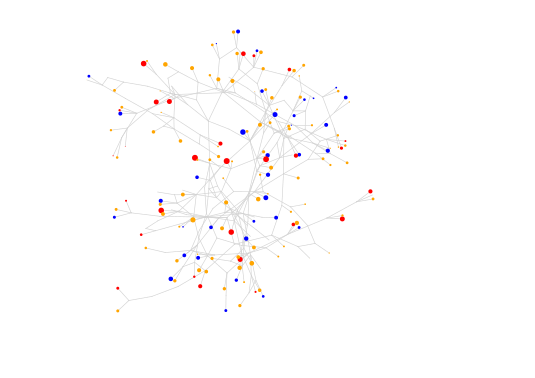
\includegraphics[width=1.4\linewidth]{fig/graph_grid.png}}
\caption{Network Grid graph}
\label{fig:graph_grid}
\end{figure}

Figure \ref{fig:graph_grid} shows the installed power available in the network (grouped by bus) using a logarithmic scale. The red nodes represent the thermal generators, the blue represent the hydro generators. For comparison purposes, orange nodes have been added that are equivalent to average real power demands.

As we can see from the plot of the grid \ref{fig:graph_grid}, this appears to be a well balanced case, with similar installed hydro and thermal power capacity and with a reasonable average demand. In addition, it is a well distributed network, without any evident critical sections susceptible to impacting power flow problems. Those facts are indications of a significant hydro-generation optimal dispatch without large complications.

For this study, a 160 stage horizon planning and simulation have been executed using the following case parameters:

\begin{itemize}
    \item Number of stages: 160
    \item Number of hours in stage: 168 
    \item Network Formulation: Linear DC approximation
\end{itemize}

\subsection{Results} %\label{subsub:results}

The simulate command returns a detailed dictionary of the execution. In order to plot those results returned by the simulate function, you may choose from a variety of methods, including the function \texttt{plot\_aggregate\_results()}. This function receives the dictionary results and generates the most common aggregated variable plots, which best summarize simulations of a hydrothermal dispatch:

\begin{lstlisting}[language = Julia]
plot_aggregated_results(results)
\end{lstlisting}

% Figures \ref{fig:plot_agg_result_thermal} to
Figures 2 to \ref{fig:plot_agg_result_inflow} show the output from the above command. As mentioned, the plots are of aggregated quantities, but the methods used to aggregate were chosen in order to help analysis. For example: the final nodal price is an average of nodal prices weighted by the contribution of local loads to the total demand; reservoir volume was grouped weighted by the amount of energy that could be produced by the stored water (as was the inflow of water).

As expected the optimal dispatch of the simulations uses more hydro-generators, however it needs thermal-generators to met all demands without deficit. On this hydro-dominated system, the uncertain inflow is a driving factor of optimal dispatch. As we can see in Figure \ref{fig:plot_agg_result_inflow}, the inflow has a strong seasonality component, resulting the significant seasonality trait observable in the variables of the policy simulations.
%\ref{fig:plot_agg_result_thermal}
2-\ref{fig:plot_agg_result_load}, \ref{fig:plot_agg_result_hydrogen}-\ref{fig:plot_agg_result_vol}.

Similar studies are possible for any case and formulation chosen, helping to analyze existing realistic cases and assess impacts of future system changes. 

% \begin{figure}[!ht]\label{fig:thermal}
% \centering
% 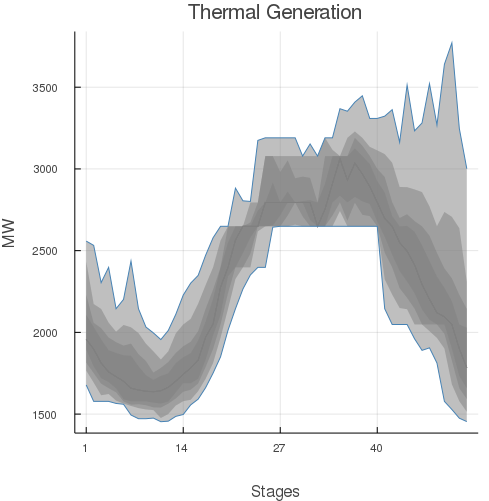
\includegraphics[width=0.5\columnwidth]{fig/plot_agg_result_thermal.png}
% \caption{Aggregated quantity of thermal generation.}
% \end{figure}

\begin{figure}[H]
\centerline{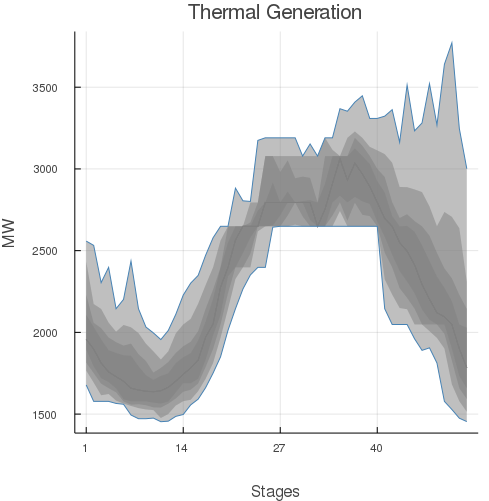
\includegraphics[width=0.5\linewidth]{fig/plot_agg_result_thermal.png}}
\label{fig:plot_agg_result_thermal}
\caption{Thermal Generation}
\end{figure}

\begin{figure}[H]
\centerline{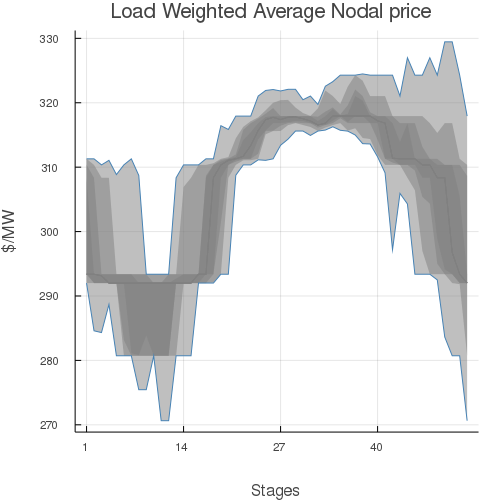
\includegraphics[width=0.55\linewidth]{fig/plot_agg_result_load.png}}
\caption{Load Weighted Average Nodal Price}
\label{fig:plot_agg_result_load}
\end{figure}

\begin{figure}[H]
\centerline{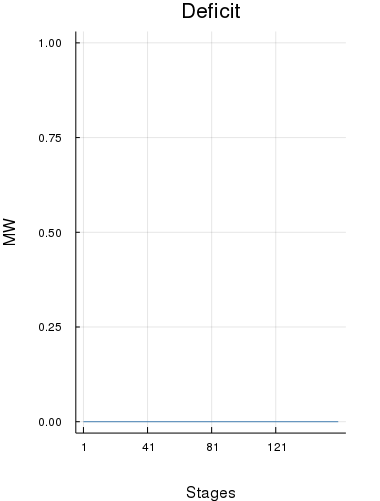
\includegraphics[width=0.55\linewidth]{fig/plot_agg_result_def.png}}
\caption{Deficit}
\label{fig:plot_agg_result_def}
\end{figure}

\begin{figure}[H]
\centerline{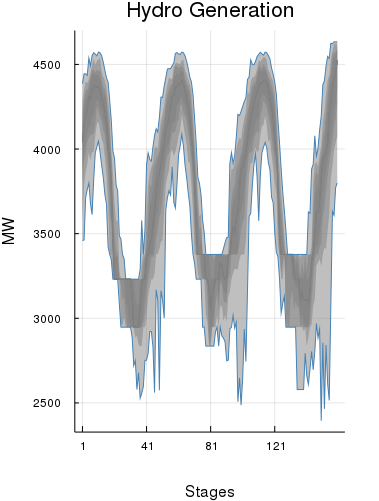
\includegraphics[width=0.55\linewidth]{fig/plot_agg_result_hydrogen.png}}
\caption{Hydro Generation}
\label{fig:plot_agg_result_hydrogen}
\end{figure}

\begin{figure}[H]
\centerline{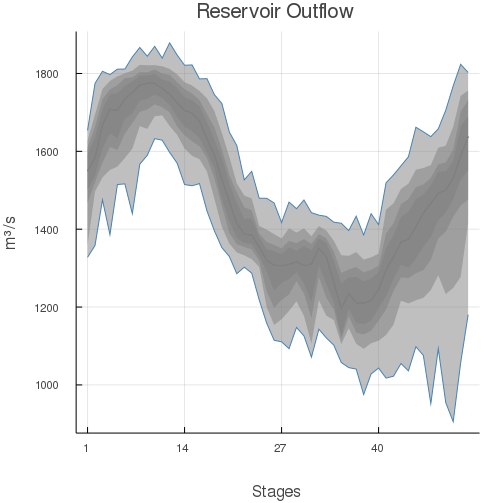
\includegraphics[width=0.55\linewidth]{fig/plot_agg_result_hydroturn.png}}
\caption{Hydro Turn (Storage Outflow)}
\label{fig:plot_agg_result_hydroturn}
\end{figure}

\begin{figure}[H]
\centerline{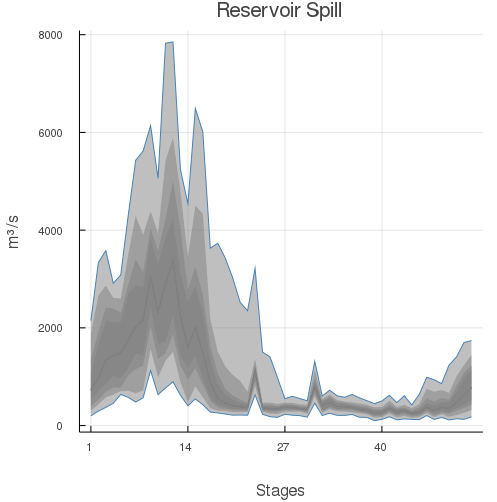
\includegraphics[width=0.5\linewidth]{fig/plot_agg_result_hydrospill.png}}
\caption{Hydro Spillage (Storage Spillage)}
\label{fig:plot_agg_result_hydrospill}
\end{figure}

\begin{figure}[H]
\centerline{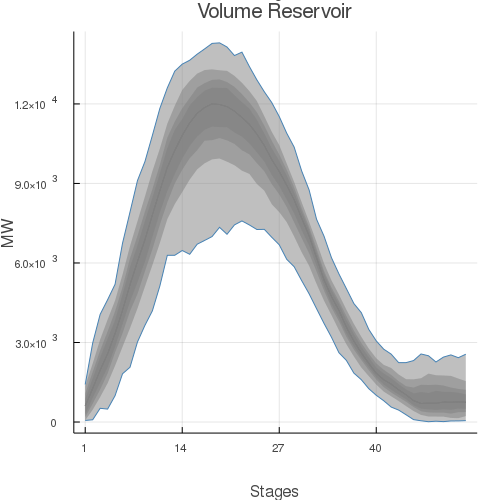
\includegraphics[width=0.55\linewidth]{fig/plot_agg_result_vol.png}}
\caption{Volume Reservoir}
\label{fig:plot_agg_result_vol}
\end{figure}

\begin{figure}[H]
\centerline{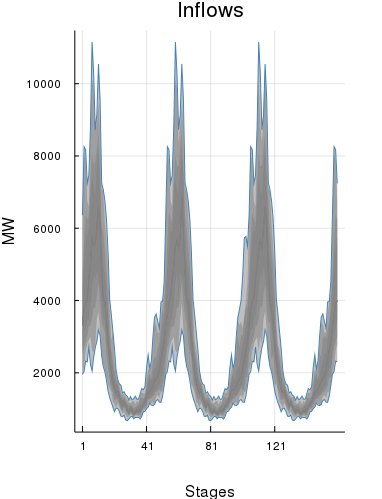
\includegraphics[width=0.55\linewidth]{fig/plot_agg_result_inflow.png}}
\caption{Inflow}
\label{fig:plot_agg_result_inflow}
\end{figure}

% **************GENERATED FILE, DO NOT EDIT**************

\bibliographystyle{juliacon}
\bibliography{ref.bib}


\end{document}

% Inspired by the International Journal of Computer Applications template

